\documentclass{manuscript}

\usepackage[hidelinks]{hyperref}
\usepackage{textcomp}
\usepackage{amsmath}
\usepackage{tikz}

\title{A Graph-based Algorithm for Finding Arbitrage Oppotunities in the Cryptocurrency Spot Market}
\author{Zhang Shiwei}
\date{October 2017}

\begin{document}
    \maketitle

    \section{Introduction}

    \subsection{Cryptocurrency Spot Market}

    Cryptocurrencys spot markets are exchanges where people trading their digital coins like Bitcoin, Ethereum, etc.
    On October 19, 2017, the market capitalizations of the top coins are shown in Table \ref{Tab:1}.\footnote{Source:\url{coinmarketcap.com}}

    \begin{table}[h]
        \centering
        \begin{tabular}{l *{4}{r}}
            Coin & Market Cap. & Price & Volume (24h) \\
            \hline
            Bitcoin & \$102,461,472,454 & \$6158.66 & \$2,708,970,000 \\
            Ethereum & \$28,154,471,164 & \$295.64 & \$451,489,000 \\
            Ripple & \$7,867,600,806 & \$0.20 & \$136,479,000 \\
            Bitcoin Cash & \$5,375,340,170 & \$321.73 & \$158,438,000 \\
            Litecoin & \$3,155,405,470 & \$59.01 & \$176,593,000 \\
            \hline
        \end{tabular}
        \caption{Cryptocurrencys market capitalizations}\label{Tab:1}
    \end{table}

    Many exchanges not only offer trading pairs between digital coins and government-issued currencies, but also support
    the trading between diffrent coins. This enables some trading strategies like triangular arbitrage.

    Another notable feature of the cryptocurrency spot market is that some exchanges charges no trading fees (e.g. OKEx),
    thus we can trade very rapidly, no matter how small the profit is.

    \subsection{Triangular Arbitrage}\label{triangular arbitrage}

    Suppose we have $x_i$ dollars. If we use them to buy some bitcoins, then use these bitcoins to buy ethereums, and
    finally sell those ethereums for $x_f$ dollars. If $x_f > x_i$, a profit is realized. Since the cryptocurrency spot
    market is active, we can expect $x_f - x_i$ is very small, and only occurs at minute or second time scale.

    Triangular arbitrage opportunities can be identified through the rate product
    \[ \gamma(t) = \prod_{i=1}^{3}r_i(t) \]
    where $r_i(t)$ denotes an exchange rate at time $t$. An arbitrage is theoretically possible if $\gamma > 1$. For each
    group of exchange rates there are two unique rate products that can be calculated. For example, consider the set of
    rates \{BTC/USD, ETH/USD, ETH/BTC\}. If one initially holds US dollars, a possible arbitrage transaction sequence is
    USD\textrightarrow{}BTC\textrightarrow{}ETH\textrightarrow{}USD with the rate product given by
    \[ \gamma_1(t) = \left[\frac{1}{\text{BTC/USD}_{ask}(t)}\right]\cdot
                     \left[\frac{1}{\text{ETH/BTC}_{ask}(t)}\right]\cdot
                     \left[\text{ETH/USD}_{bid}(t)\right] \]
    and the rate product of the other possible trading sequence is
    \[ \gamma_2(t) = \left[\text{BTC/USD}_{bid}(t)\right]\cdot
                     \left[\text{ETH/BTC}_{bid}(t)\right]\cdot
                     \left[\frac{1}{\text{ETH/USD}_{ask}(t)}\right] \]
    These two rate products define all possible arbitrage transactions using this set of trading pairs.\cite{fenn2009mirage}

    \subsection{Inter-market Arbitrage}

    Suppose there are two exchange $E_1$ and $E_2$ offering the same trading pair ETH/BTC with price $ask_i(t)$ and $bid_i(t)$
    at time $t$, where $i = {1,2}$. An inter-market arbitrage strategy can be buying ETH with BTC in $E_1$ and sell them
    for BTC in $E_2$. If $ask_1(t) < bid_2(t)$ and you managed to trade at both price, a profit $bid_2(t) - ask_1(t)$
    then got realized.

    This is pretty similar with the triangular arbitrage described in section \ref{triangular arbitrage}. In fact, we can
    assume there being two implict trading pair between $\text{BTC}_{E_1} \text{/} \text{BTC}_{E_2}$ with both ask and
    bid price always being 1 (or minus transferring fee rates). The Inter-market arbitrage then become a ``quadrangle arbitrage''
    with all theorems the same as triangular arbitrage except for there being 4 nodes.

    \subsection{Graph Algorithms}

    In graph theory, graphs are mathematical structures used to model pairwise relations between objects. A graph in this
    context is made up of nodes and paths. A weight can be attached to nodes and/or paths. The following figure shows a
    drawing of a directed graph.

    \begin{figure}[h]
        \centering
        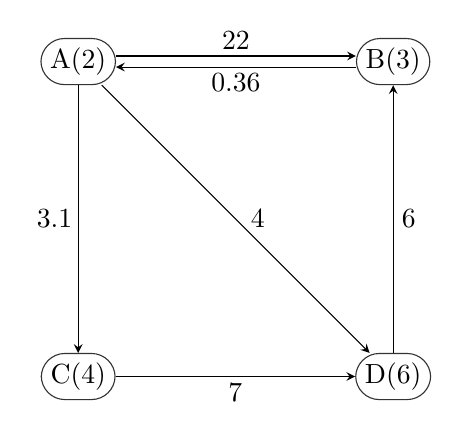
\begin{tikzpicture}[
                > = stealth,
                node/.style={ rectangle, rounded corners = 3mm, draw = black!80 },
                up/.style={ ->, transform canvas={yshift=.7mm} },
                down/.style={ ->, transform canvas={yshift=-.7mm} }
            ]
            \node (A) [node] at (0, 4) {A(2)};
            \node (B) [node] at (4, 4) {B(3)};
            \node (C) [node] at (0, 0) {C(4)};
            \node (D) [node] at (4, 0) {D(6)};

            \draw [up]   (A) -> node[yshift=2mm]{22}    (B);
            \draw [down] (B) -> node[yshift=-2mm]{0.36} (A);
            \draw [->]   (A) -> node[xshift=-3mm]{3.1}  (C);
            \draw [->]   (D) -> node[xshift=2mm]{6}     (B);
            \draw [->]   (C) -> node[yshift=-2mm]{7}    (D);
            \draw [->]   (A) -> node[xshift=1.4mm, xshift=1.4mm]{4} (D);
        \end{tikzpicture}
        \caption{A directed graph with weights both on nodes and paths}\label{Fig:1}
    \end{figure}

    There are many mature algorithm can be performed on graphs, like finding the shortest (in terms of the sum of weights
    of paths) path between two nodes with Floyd-Warshall algorithm or enumerating strongly connected components with
    Tarjan's algorithm.

    \section{Coinflow}

    \subsection{The Idea}

    We can think of our assets in $(exchange, coin)$ as nodes in a graph and exchange pairs as paths indicating methods
    through which we can transfer our assets from one node to another with a rate. For example, if there is a bid order
    of LTC/BTC with price 0.008 and fee 0.1\% in OKEx, we can draw a line from $(OKEx, LTC)$ to $(OKEx, BTC)$ with weight
    0.007992 since you can sell 1 LTC on OKEx and get 0.007992 BTC by filling that order. There are also paths with weight
    1 between diffrent exchanges with the same coin since we can withdraw the coins from one exchange and deposit to another
    with only constant fee (and almost ignorable).

    With these nodes and paths, we get a graph where our assets can flow from exchanges and coins types with operations
    (trading or transfering). Then we can try to find circles in this graph where the product of paths' weights > 1. For
    example,




    \subsection{Details}

    \section{Experiments}
    \section{Disscussion}


    \bibliographystyle{apalike}%unsrt
    \bibliography{main}

\end{document}
